\documentclass{article}
\usepackage[portuguese]{babel}
\usepackage[utf8]{inputenc}
\usepackage{graphicx}
\usepackage{booktabs}
\usepackage{hyperref}
\usepackage{verbatim}

\title{Análise de Dados de Vinhos Portugueses}
\author{Seu Nome}
\date{Data do Relatório}

\begin{document}

\maketitle

\begin{abstract}
Este relatório apresenta uma análise de vinhos portugueses ``Vinho Verde'' e modelos de machine learning para previsão de qualidade e teor alcoólico, bem como a distinção entre vinhos tintos e brancos.
\end{abstract}

\section{Introdução}
Introdução ao projeto e aos conjuntos de dados.

\section{Análise Exploratória de Dados}

\subsection{Visão Geral Rápida}
Esta subsecção apresenta uma visão geral inicial dos conjuntos de dados. O código a seguir foi utilizado para carregar e inspecionar os dados:

\begin{verbatim}
def load_data():
  home = Path.home()
  red_raw_path = home / "Desktop" / "56870" / "code" / "data" / "raw" / "red_wine.csv"
  white_raw_path = home / "Desktop" / "56870" / "code" / "data" / "raw" / "white_wine.csv"

  red_wine = pd.read_csv(red_raw_path)
  white_wine = pd.read_csv(white_raw_path)
  return red_wine, white_wine
\end{verbatim}

Ao carregar os dados foi possível observar que os conjuntos de dados possuem 12 colunas cada (acidez fixa, acidez volátil, ácido cítrico, açúcar residual, cloretos, dióxido de enxofre livre, dióxido de enxofre total, densidade, pH, sulfatos, álcool, qualidade).

As colunas de atributos são todas numéricas. Os valores s#ao todos float64 ou int32.

Foi feito uma inspecao rapida onde se encontrou que havia outliers em algumas colunas, e três valores nulos no conjunto de dados de vinhos brancos e vermelhos.

Como a imagem abaixo mostra, no vinho branco, na acidez fixa, existem um caso desses outliers:

\begin{figure}[ht]
  \centering
  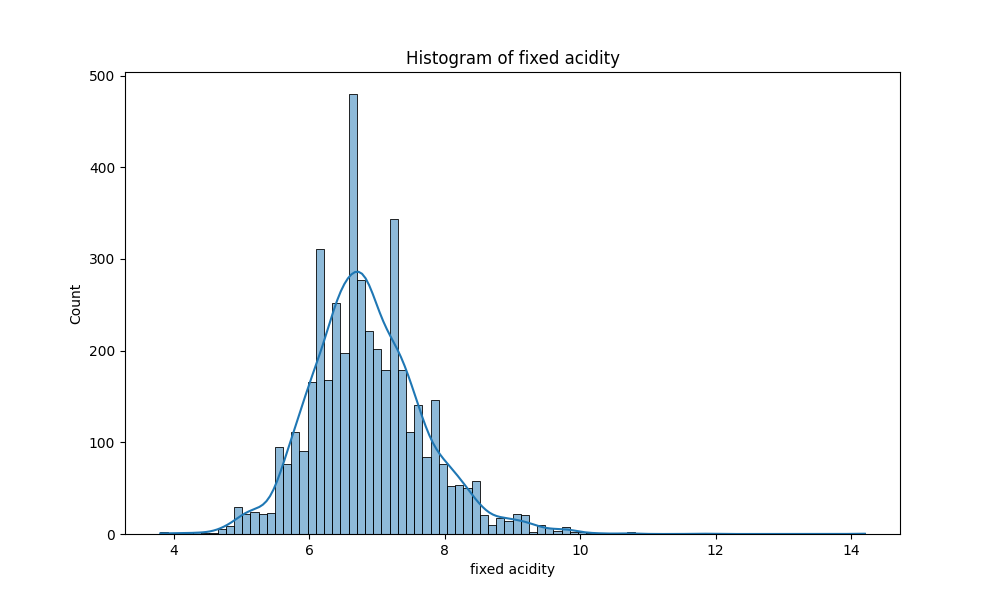
\includegraphics[width=0.8\textwidth]{../out/graphs/white_fixed_acidity_histogram.png}
  \caption{Outliers na acidez fixa do vinho branco.}
  \label{fig:outliers_white_fixed_acidity}
\end{figure}

\begin{verbatim}
def show_null_values(df):
  print("Null Values in Each Column:")
  print(df.isnull().sum())

def show_outliers(df):
  print("Outliers in Each Column: ")
  print(df.quantile([0.05, 0.95]))
  for col in df.columns:
      print(col)
      print(df[col].value_counts())
\end{verbatim}

\subsection{Valores Nulos ou Ausentes}
Tratamos da presença de valores nulos ou ausentes nos conjuntos de dados utilizando o seguinte código:

\begin{verbatim}
  def parse_and_clean(data):
  for col in data.columns:
      if data[col].dtype == "object":
          data[col] = data[col].astype("str")
      elif data[col].dtype == "int":
          data[col] = data[col].astype("int32")
      else:
          data[col] = data[col].astype("float64")

  data.replace([None, "", "NaN"], pd.NA, inplace=True)
  return data
\end{verbatim}

Este método converte os tipos de dados para os tipos mais adequados e substitui valores nulos ou ausentes por \texttt{pd.NA}.

Com isso, foi possível observar que os conjuntos de dados não possuem mais valores nulos ou ausentes. O valor \texttt{pd.NA} já é um valor nulo, mas é tratado de forma diferente pelo pandas. Com isto em mente, podemos dizer que os conjuntos de dados não possuem mais valores nulos ou ausentes (os quais possam dar problemas na análise).

\subsection{Detecção de Outliers e Tratamento}
Para identificar e tratar outliers, utilizamos o seguinte método:

\begin{verbatim}
  def handle_outliers(data):
  for col in data.select_dtypes(include=["float64", "int32"]):
      data[col] = winsorize(data[col], limits=[0.05, 0.05])
  return data
\end{verbatim}

Este método utiliza a função \texttt{winsorize} da biblioteca \texttt{scipy.stats} para substituir os outliers por valores próximos aos limites do intervalo de confiança.

\texttt{Winsorize} é uma função que recebe um array e retorna um array com os outliers substituídos. O parâmetro \texttt{limits} é um tuple que define os limites do intervalo de confiança. Neste caso, os limites são 0.05 e 0.95, o que significa que os valores abaixo do percentile 5 e acima do percentile 95 serão substituídos.

O tratamento dos tipos de dados já está incluído na função parse_and_clean, ao qual foi força a conversão de todos os valores para o tipo correto.

\subsection{Normalização dos Dados}
Para normalizar os dados, utilizamos o seguinte método:

\begin{verbatim}
def normalize_data(data):
  scaler = RobustScaler()
  scaled_data = pd.DataFrame(
      scaler.fit_transform(data), columns=data.columns)
  return scaled_data
\end{verbatim}

Ao usar o \texttt{RobustScaler}, os dados são normalizados usando a seguinte fórmula:

\begin{equation}
  X_{scaled} = \frac{X - Q_1(X)}{Q_3(X) - Q_1(X)}
\end{equation}

Onde $Q_1(X)$ é o primeiro quartil e $Q_3(X)$ é o terceiro quartil.
Este metodo por si já trata os outliers, pois o \texttt{RobustScaler} é um método robusto, no entanto, foi utilizado o método \texttt{handle\_outliers} para garantir que os outliers fossem tratados antes da normalização.

É tambem resistentes a \textit{pd.NA}.

\subsection{Fusão e Exportação dos Dados Tratados}
Os conjuntos de dados tratados foram combinados e exportados usando o seguinte código:

\begin{verbatim}
def merge_datasets(red_wine, white_wine):
  red_wine["type"] = "red"
  white_wine["type"] = "white"
  merged_wine = pd.concat([red_wine, white_wine], ignore_index=True)
  return merged_wine
\end{verbatim}

E para exportar os dados:

\begin{verbatim}
  red_wine.to_csv(red_export_path, index=False)
  white_wine.to_csv(white_export_path, index=False)
  merged_wine.to_csv(merged_export_path, index=False)
\end{verbatim}

\section{Análise Exploratória de Dados}

Ainda no mesmo script, foram feitas algumas análises exploratórias de dados. A seguir, apresentamos os resultados.

\subsection{Distribuição de Atributos}
A distribuição de atributos foi analisada usando o seguinte código:

\begin{verbatim}
  def eda(data, wine_type):
  print(data.describe())

  for col in data.columns:
      sns.histplot(data[col], kde=True)
      plt.title(f'Histogram of {col}')

  fig_save_path = Path.home() / "Desktop" / "56870" / "code" / "data" / "out" / "graphs" / f"{wine_type}_analysis.png"
  fig_save_path.parent.mkdir(parents=True, exist_ok=True)
  plt.savefig(fig_save_path)
\end{verbatim}

O método \texttt{describe} retorna um resumo estatístico dos dados. O método \texttt{histplot} da biblioteca \texttt{seaborn} gera um histograma para cada coluna do conjunto de dados.

Aqui o eda foi chamado duas vezes, uma para cada conjunto de dados. Os resultados foram salvos em \texttt{out/graphs}.

\subsection{Correlação entre Atributos}
A correlação entre atributos foi analisada usando o seguinte código:

\begin{verbatim}
def correlation(data, wine_type):
  corr = data.corr()
  sns.heatmap(corr, annot=True)
  plt.title(f'Correlation Heatmap of {wine_type} Wine')
  fig_save_path = Path.home() / "Desktop" / "56870" / "code" / "data" / "out" / "graphs" / f"{wine_type}_correlation.png"
  fig_save_path.parent.mkdir(parents=True, exist_ok=True)
  plt.savefig(fig_save_path)
\end{verbatim}

O método \texttt{corr} da biblioteca \texttt{pandas} retorna uma matriz de correlação entre os atributos. O método \texttt{heatmap} da biblioteca \texttt{seaborn} gera um mapa de calor para a matriz de correlação.

O gráfico de correlação gerado para os vinhos tintos é apresentado na Figura \ref{fig:corr_red} e o gráfico de correlação gerado para os vinhos brancos é apresentado na Figura \ref{fig:corr_white}.

\begin{figure}[ht]
  \centering
  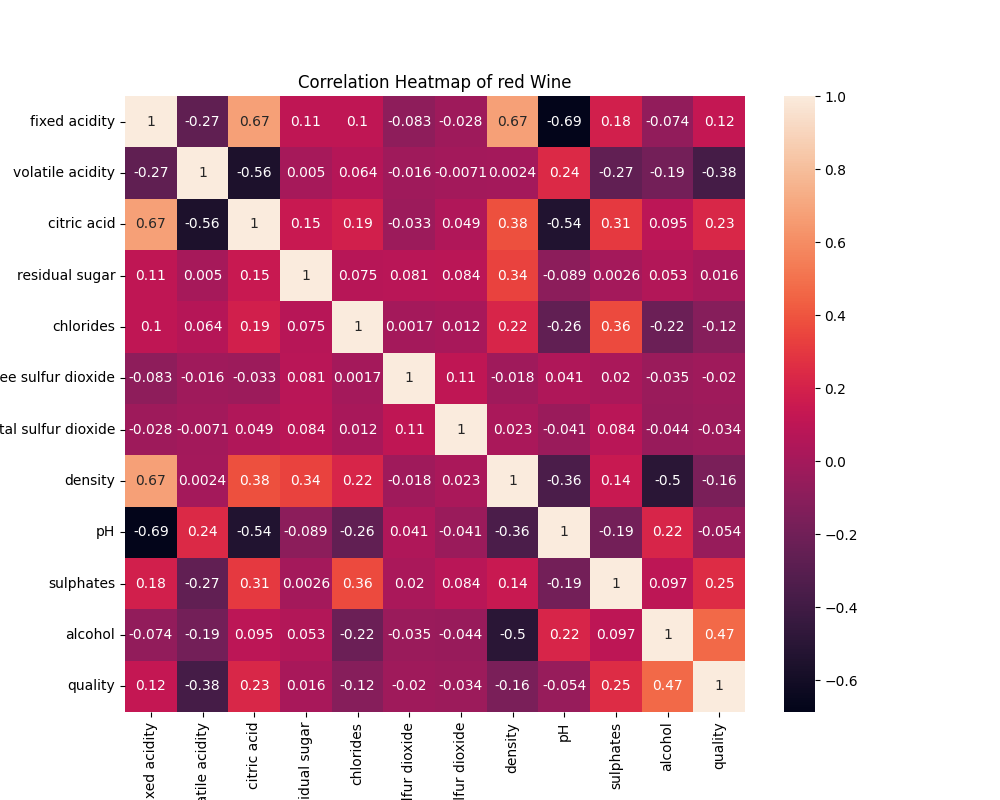
\includegraphics[width=0.8\textwidth]{../out/graphs/red_correlation.png}
  \caption{Mapa de calor da correlação entre os atributos dos vinhos tintos.}
  \label{fig:corr_red}
\end{figure}

\begin{figure}[ht]
  \centering
  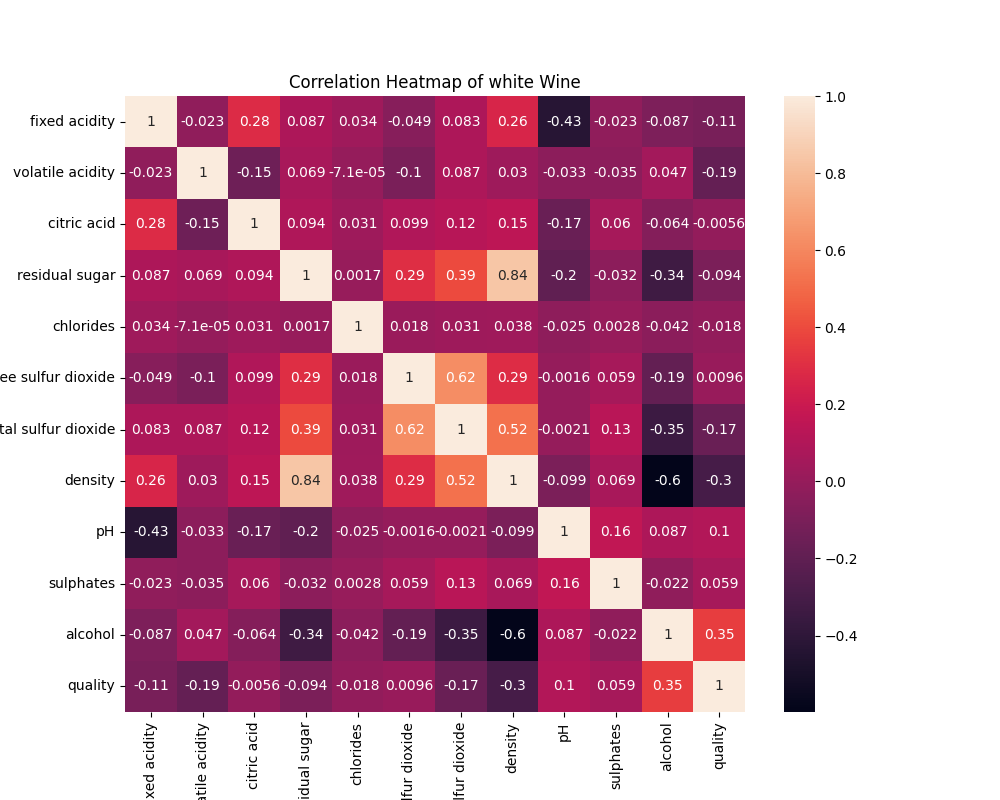
\includegraphics[width=0.8\textwidth]{../out/graphs/white_correlation.png}
  \caption{Mapa de calor da correlação entre os atributos dos vinhos brancos.}
  \label{fig:corr_white}
\end{figure}

Como podemos observar, os atributos mais correlacionados com a qualidade são o álcool e a acidez volátil. Os atributos mais correlacionados com o álcool são a densidade e o açúcar residual. Os atributos mais correlacionados com a acidez volátil são o ácido cítrico e o pH.

\section{Tarefa de Regressão}

Com esta tarefa, pretendemos prever o nível de álcool dos vinhos através dos outros atributos com modelos de regressão.

\subsection{Previsão de nível de álcool}
Para prever o nível de álcool, utilizamos os seguintes modelos:

\begin{enumerate}
  \item Regressão Linear
  \item Regressão de Floresta Aleatória
\end{enumerate}

Os quais foram implementados usando o seguinte código:

\begin{verbatim}
  x = data.drop('alcohol', axis=1)
  y = data['alcohol']
  x_train, x_test, y_train, y_test = train_test_split(x, y, test_size=0.2, random_state=42)

  lr = LinearRegression()
  lr.fit(x_train, y_train)
  y_pred = lr.predict(x_test)
  print("Linear Regression MSE:", mean_squared_error(y_test, y_pred))
  print("Linear Regression R2 Score:", r2_score(y_test, y_pred))
  print("Linear Regression MAE:", mean_absolute_error(y_test, y_pred))
  save_model(lr, 'task1_linear_regression_alcohol.pk1')

  rf = RandomForestRegressor()
  rf.fit(x_train, y_train)
  y_pred_rf = rf.predict(x_test)
  print("Random Forest Regressor MSE:", mean_squared_error(y_test, y_pred_rf))
  print("Random Forest Regressor R2 Score:", r2_score(y_test, y_pred_rf))
  print("Random Forest Regressor MAE:", mean_absolute_error(y_test, y_pred_rf))
  save_model(rf, 'task1_random_forest_alcohol.pk1')
\end{verbatim}

O output do código acima é apresentado a seguir:

\begin{verbatim}
  Linear Regression MSE: 0.11231851016651878
Linear Regression R2 Score: 0.7099030226588107
Linear Regression MAE: 0.2594028031889842
Random Forest Regressor MSE: 0.05065648568715602
Random Forest Regressor R2 Score: 0.8691640998550947
Random Forest Regressor MAE: 0.15210464478057667
\end{verbatim}

Ou seja.

Com estes modelos, obtivemos os seguintes resultados:

\begin{table}[ht]
  \centering
  \begin{tabular}{@{}lll@{}}
    \toprule
    Modelo & MSE & R2 Score \\ \midrule
    Regressão Linear & 0.11 & 0.71 \\
    Regressão de Floresta Aleatória & 0.05 & 0.87 \\ \bottomrule
  \end{tabular}
  \caption{Resultados da tarefa de regressão.}
  \label{tab:task1_results}
\end{table}

Com base nos resultados apresentados na Tabela \ref{tab:task1_results}, podemos concluir que o modelo de regressão de floresta aleatória é o mais adequado para prever o nível de álcool. Este modelo obteve um MSE de 0.05 e um R2 Score de 0.87, enquanto que o modelo de regressão linear obteve um MSE de 0.11 e um R2 Score de 0.71.

Não só sendo melhor na previsão como tambem nos proporciona a a oportunidade de analisar a importancia de cada atributo para a previsão.

\begin{figure}[ht]
  \centering
  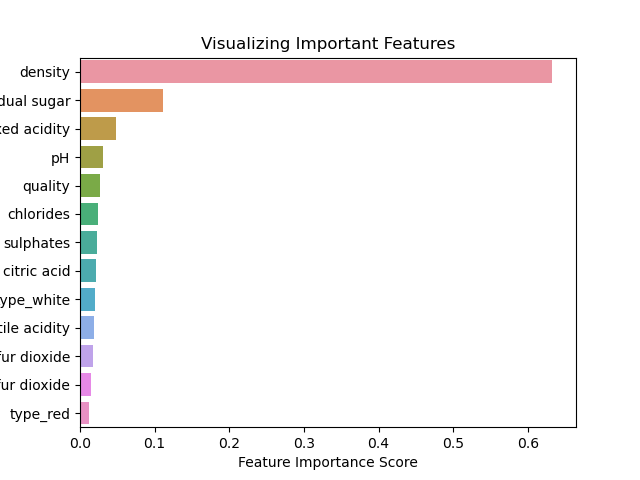
\includegraphics[width=0.8\textwidth]{../out/graphs/feature_importance.png}
  \caption{Importância dos atributos para a previsão do nível de álcool.}
  \label{fig:task1_feature_importance}
\end{figure}

Como podemos observar na Figura \ref{fig:task1_feature_importance}, os atributos mais importantes para a previsão do nível de álcool são a densidade, o açúcar residual e o pH.

\section{Tarefa de Classificação}

Com esta tarefa, pretendemos prever o tipo de vinho (tinto ou branco) através dos outros atributos com modelos de classificação.

\subsection{Previsão do tipo de vinho}

Para prever o tipo de vinho, utilizamos os seguintes modelos:

\begin{enumerate}
  \item Regressão Logística
  \item Floresta Aleatória
\end{enumerate}

Os quais foram implementados usando o seguinte código:

\begin{verbatim}
  x = data.drop('type', axis=1)
  y = data['type']
  x_train, x_test, y_train, y_test = train_test_split(x, y, test_size=0.2, random_state=42)

  fix_score = 'red'

  log_reg = LogisticRegression()
  log_reg.fit(x_train, y_train)
  y_pred = log_reg.predict(x_test)
  print("Logistic Regression Accuracy:", accuracy_score(y_test, y_pred))
  print("Logistic Regression F1 Score:", f1_score(y_test, y_pred, pos_label=fix_score))
  print("Logistic Regression Precision:", precision_score(y_test, y_pred, pos_label=fix_score))
  print("Logistic Regression Recall:", recall_score(y_test, y_pred, pos_label=fix_score))
  save_model(log_reg, 'task2_logistic_regression_type.pk1')

  rfc = RandomForestClassifier()
  rfc.fit(x_train, y_train)
  y_pred_rfc = rfc.predict(x_test)
  print("Random Forest Classifier Accuracy:", accuracy_score(y_test, y_pred_rfc))
  print("Random Forest Classifier F1 Score:", f1_score(y_test, y_pred_rfc, pos_label=fix_score))
  print("Random Forest Classifier Precision:", precision_score(y_test, y_pred_rfc, pos_label=fix_score))
  print("Random Forest Classifier Recall:", recall_score(y_test, y_pred_rfc, pos_label=fix_score))
  save_model(rfc, 'task2_random_forest_type.pk1')
\end{verbatim}

O output do código acima é apresentado a seguir:

\begin{verbatim}
  Logistic Regression Accuracy: 0.7735042735042735
  Logistic Regression F1 Score: 0.32569974554707376
  Logistic Regression Precision: 0.7272727272727273
  Logistic Regression Recall: 0.2098360655737705
  Random Forest Classifier Accuracy: 0.9726495726495726
  Random Forest Classifier F1 Score: 0.9446366782006921
  Random Forest Classifier Precision: 1.0
  Random Forest Classifier Recall: 0.8950819672131147
\end{verbatim}

Ou seja.

Com estes modelos, obtivemos os seguintes resultados:

\begin{table}[ht]
  \centering
  \begin{tabular}{@{}lllll@{}}
    \toprule
    Modelo & Accuracy & F1 Score & Precisão & Recall \\ \midrule
    Regressão Logística & 0.77 & 0.33 & 0.73 & 0.21 \\
    Floresta Aleatória & 0.97 & 0.94 & 1.0 & 0.90 \\ \bottomrule
  \end{tabular}
  \caption{Resultados da tarefa de classificação.}
  \label{tab:task2_results}
\end{table}

E temos que a matriz de confusão para o modelo de floresta aleatória é a seguinte:

\begin{figure}[ht]
  \centering
  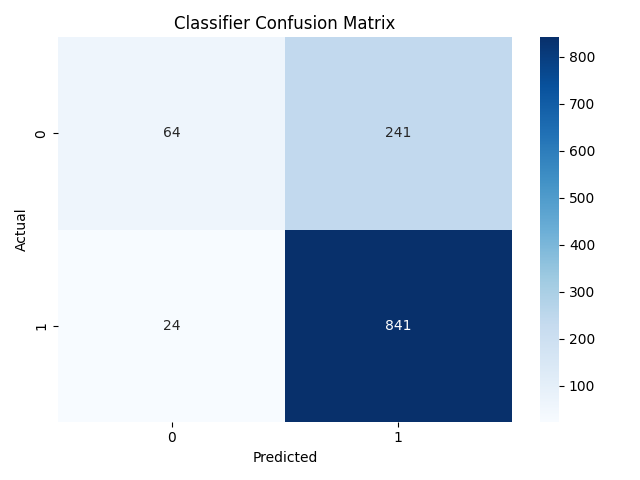
\includegraphics[width=0.8\textwidth]{../out/graphs/task2_log_reg_matrix.png}
  \caption{Matriz de confusão para o modelo de floresta aleatória.}
  \label{fig:task2_confusion_matrix}
\end{figure}

E para o modelo de regressão logística:

\begin{figure}[ht]
  \centering
  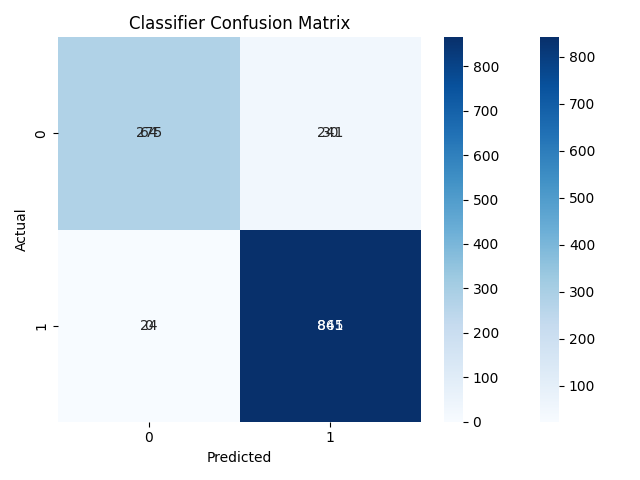
\includegraphics[width=0.8\textwidth]{../out/graphs/task2_rfc_matrix.png}
  \caption{Matriz de confusão para o modelo de regressão logística.}
  \label{fig:task2_confusion_matrix}
\end{figure}

Com base nos resultados apresentados na Tabela~\ref{tab:task2_results}, podemos concluir que o modelo de floresta aleatória é o mais adequado para prever o tipo de vinho. Este modelo obteve uma \textit{accuracy} de 0.97, um F1 Score de 0.94, uma precisão de 1.0 e um \textit{recall} de 0.90, enquanto que o modelo de regressão logística obteve uma \textit{accuracy} de 0.77, um F1 Score de 0.33, uma precisão de 0.73 e um \textit{recall} de 0.21.

Continuando a moda anterior dos modelos de floresta aleatória serem os melhores para este caso de estudo especifico.

\begin{figure}[ht]
  \centering
  \includegraphics[width=0.8\textwidth]{../out/graphs/confusion_matrix.png}
  \caption{Matriz de confusão para o modelo de floresta aleatória.}
  \label{fig:task2_confusion_matrix}
\end{figure}

\section{Tarefa de previsão de qualidade}

Com esta tarefa, pretendemos prever a qualidade dos vinhos através dos outros atributos com modelos de classificação.

\subsection{Previsão da qualidade dos vinhos}

Para prever a qualidade dos vinhos, utilizamos os seguintes modelos:

\begin{enumerate}
  \item \textit{Gradient Boosting Regressor}
  \item \textit{K-Nearest Neighbors Regressor}
  \item \textit{Linear Regression}
  \item \textit{Random Forest Regressor}
  \item \textit{Support Vector Regressor}
\end{enumerate}

Os quais foram implementados usando o seguinte código:

\begin{verbatim}
  lr = LinearRegression()
  lr.fit(x_train, y_train)
  y_pred_lr = lr.predict(x_test)
  print("Linear Regression MSE:", mean_squared_error(y_test, y_pred_lr))
  print("Linear Regression R2 Score:", r2_score(y_test, y_pred_lr))
  print("Linear Regression MAE:", mean_absolute_error(y_test, y_pred_lr))
  save_model(lr, 'task3_linear_regression_quality.pk1')

  gbr = GradientBoostingRegressor()
  gbr.fit(x_train, y_train)
  y_pred_gbr = gbr.predict(x_test)
  print("Gradient Boosting Regressor MSE:", mean_squared_error(y_test, y_pred_gbr))
  print("Gradient Boosting Regressor R2 Score:", r2_score(y_test, y_pred_gbr))
  print("Gradient Boosting Regressor MAE:", mean_absolute_error(y_test, y_pred_gbr))
  save_model(gbr, 'task3_gradient_boosting_quality.pk1')

  knn = KNeighborsRegressor()
  knn.fit(x_train, y_train)
  y_pred_knn = knn.predict(x_test)
  print("KNN Regressor MSE:", mean_squared_error(y_test, y_pred_knn))
  print("KNN Regressor R2 Score:", r2_score(y_test, y_pred_knn))
  print("KNN Regressor MAE:", mean_absolute_error(y_test, y_pred_knn))
  save_model(knn, 'task3_knn_quality.pk1')

  svr = SVR()
  svr.fit(x_train, y_train)
  y_pred_svr = svr.predict(x_test)
  print("SVR MSE:", mean_squared_error(y_test, y_pred_svr))
  print("SVR R2 Score:", r2_score(y_test, y_pred_svr))
  print("SVR MAE:", mean_absolute_error(y_test, y_pred_svr))
  save_model(svr, 'task3_svr_quality.pk1')

  rf = RandomForestRegressor()
  rf.fit(x_train, y_train)
  y_pred_rf = rf.predict(x_test)
  print("Random Forest Regressor MSE:", mean_squared_error(y_test, y_pred_rf))
  print("Random Forest Regressor R2 Score:", r2_score(y_test, y_pred_rf))
  print("Random Forest Regressor MAE:", mean_absolute_error(y_test, y_pred_rf))
  save_model(rf, 'task3_random_forest_quality.pk1')
\end{verbatim}

O output do código acima é apresentado a seguir:

\begin{verbatim}
  Linear Regression MSE: 0.3791330547891043
  Linear Regression R2 Score: 0.27383190985246364
  Linear Regression MAE: 0.508457234349973
  Gradient Boosting Regressor MSE: 0.3294945025105814
  Gradient Boosting Regressor R2 Score: 0.3689065340522302
  Gradient Boosting Regressor MAE: 0.47205398588447034
  KNN Regressor MSE: 0.3535384615384615
  KNN Regressor R2 Score: 0.3228542165707762
  KNN Regressor MAE: 0.46273504273504273
  SVR MSE: 0.329904406833089
  SVR R2 Score: 0.3681214285720864
  SVR MAE: 0.44742076150170534
  Random Forest Regressor MSE: 0.2580932478632479
  Random Forest Regressor R2 Score: 0.5056640973046184
  Random Forest Regressor MAE: 0.39195726495726496
\end{verbatim}

Ou seja.

Com estes modelos, obtivemos os seguintes resultados:

\begin{table}[ht]
  \centering
  \begin{tabular}{@{}llll@{}}
    \toprule
    Modelo & MSE & R2 Score & MAE \\ \midrule
    \textit{Gradient Boosting Regressor} & 0.33 & 0.37 & 0.47 \\
    \textit{K-Nearest Neighbors Regressor} & 0.35 & 0.32 & 0.46 \\
    \textit{Linear Regression} & 0.37 & 0.27 & 0.50 \\
    \textit{Random Forest Regressor} & 0.26 & 0.51 & 0.39 \\
    \textit{Support Vector Regressor} & 0.32 & 0.37 & 0.44 \\ \bottomrule
  \end{tabular}
  \caption{Resultados da tarefa de previsão de qualidade.}
  \label{tab:task3_results}
\end{table}

Com base nos resultados apresentados na Tabela~\ref{tab:task3_results}, podemos concluir que o modelo de floresta aleatória é o mais adequado para prever a qualidade dos vinhos. Este modelo obteve um MSE de 0.26, um R2 Score de 0.51 e um MAE de 0.39, enquanto que os outros modelos obtiveram um MSE entre 0.32 e 0.37, um R2 Score entre 0.27 e 0.37 e um MAE entre 0.44 e 0.50.

A \textit{trend} continua, o modelo de floresta aleatória é o melhor para este caso de estudo.

\section{Conclusão}
Nesta secção, apresentamos as conclusões do projeto.

\subsection{Conclusões}
Foi efetuada uma análise exploratória de dados e foram implementados modelos de machine learning para previsão de qualidade e teor alcoólico, bem como a distinção entre vinhos tintos e brancos. Os modelos de floresta aleatória foram os mais adequados para prever o teor alcoólico, o tipo de vinho e a qualidade dos vinhos.

\subsection{Limitações}

Dada a escolha limitada da nossa parte sobre os modelos e pre-processamento dos dados, não podemos afirmar que os modelos escolhidos são os melhores para este caso de estudo. É de facto estraordinário que os modelos de floresta aleatória tenham sido os melhores para todos os casos, mas não podemos afirmar que são os melhores para este caso de estudo em especifico sem ter feito uma análise mais profunda.

\subsection{Trabalho Futuro}

Para trabalhos futuros, recomendamos que sejam feitas análises mais profundas sobre os modelos e pre-processamento dos dados. Também recomendamos que sejam feitas análises mais profundas sobre os conjuntos de dados, para que seja possível identificar possíveis problemas e limitações. É aconselhavel tambem usar uma \textit{framework} mais robusta como o PyTorch ou TensorFlow e criar modelos mais complexos e \textit{tailored} para este caso de estudo.

\section{Referências}
Bibliografia e referências utilizadas.

\end{document}
